\documentclass{scrartcl}  % scrartcl of scrreprt
\usepackage{SIunits}
% Include all project wide packages here.
\usepackage{fullpage}
\usepackage{polyglossia}
\setmainlanguage{dutch}
\usepackage{csquotes}
\usepackage{graphicx}
\usepackage{epstopdf}
\usepackage{pdfpages}
\usepackage{caption}
\usepackage[list=true]{subcaption}
\usepackage{float}
%\usepackage{mathtools}
\usepackage{standalone}
\usepackage{import}
\usepackage{tocloft}
\usepackage{wrapfig}
\usepackage{authblk}
\usepackage{array}
\usepackage{booktabs}
\usepackage[toc,page,title,titletoc]{appendix}
\usepackage{xunicode}
\usepackage{amsmath}
\usepackage{fontspec}
\usepackage{unicode-math}
\usepackage[
    backend=bibtexu,
	texencoding=utf8,
bibencoding=utf8,
    style=ieee,
    sortlocale=nl_NL,
    language=auto
]{biblatex}
\usepackage{listings}
\newcommand{\includecode}[3][c]{\lstinputlisting[caption=#2, escapechar=, style=#1]{#3}}
\newcommand{\superscript}[1]{\ensuremath{^{\textrm{#1}}}}
\newcommand{\subscript}[1]{\ensuremath{_{\textrm{#1}}}}


\newcommand{\chapternumber}{\thechapter}
\renewcommand{\appendixname}{Bijlage}
\renewcommand{\appendixtocname}{Bijlagen}
\renewcommand{\appendixpagename}{Bijlagen}

\usepackage[hidelinks]{hyperref} %<--------ALTIJD ALS LAATSTE
  
\renewcommand{\familydefault}{\sfdefault}

\setmainfont[Ligatures=TeX]{Myriad Pro}
\setmathfont{Asana Math}
\setmonofont{Lucida Console}

\usepackage{titlesec, blindtext, color}
\definecolor{gray75}{gray}{0.75}
\newcommand{\hsp}{\hspace{20pt}}
\titleformat{\chapter}[hang]{\Huge\bfseries}{\chapternumber\hsp\textcolor{gray75}{|}\hsp}{0pt}{\Huge\bfseries}
\renewcommand{\familydefault}{\sfdefault}
\renewcommand{\arraystretch}{1.2}
\setlength\parindent{0pt}

%For code listings
\definecolor{black}{rgb}{0,0,0}
\definecolor{browntags}{rgb}{0.65,0.1,0.1}
\definecolor{bluestrings}{rgb}{0,0,1}
\definecolor{graycomments}{rgb}{0.4,0.4,0.4}
\definecolor{redkeywords}{rgb}{1,0,0}
\definecolor{bluekeywords}{rgb}{0.13,0.13,0.8}
\definecolor{greencomments}{rgb}{0,0.5,0}
\definecolor{redstrings}{rgb}{0.9,0,0}
\definecolor{purpleidentifiers}{rgb}{0.01,0,0.01}


\lstdefinestyle{csharp}{
language=[Sharp]C,
showspaces=false,
showtabs=false,
breaklines=true,
showstringspaces=false,
breakatwhitespace=true,
escapeinside={(*@}{@*)},
columns=fullflexible,
commentstyle=\color{greencomments},
keywordstyle=\color{bluekeywords}\bfseries,
stringstyle=\color{redstrings},
identifierstyle=\color{purpleidentifiers},
basicstyle=\ttfamily\small}

\lstdefinestyle{c}{
language=C,
showspaces=false,
showtabs=false,
breaklines=true,
showstringspaces=false,
breakatwhitespace=true,
escapeinside={(*@}{@*)},
columns=fullflexible,
commentstyle=\color{greencomments},
keywordstyle=\color{bluekeywords}\bfseries,
stringstyle=\color{bluestrings},
identifierstyle=\color{purpleidentifiers}
}

\lstdefinestyle{vhdl}{
language=VHDL,
showspaces=false,
showtabs=false,
breaklines=true,
showstringspaces=false,
breakatwhitespace=true,
escapeinside={(*@}{@*)},
columns=fullflexible,
commentstyle=\color{greencomments},
keywordstyle=\color{bluekeywords}\bfseries,
stringstyle=\color{redstrings},
identifierstyle=\color{purpleidentifiers}
}

\lstdefinestyle{xaml}{
language=XML,
showspaces=false,
showtabs=false,
breaklines=true,
showstringspaces=false,
breakatwhitespace=true,
escapeinside={(*@}{@*)},
columns=fullflexible,
commentstyle=\color{greencomments},
keywordstyle=\color{redkeywords},
stringstyle=\color{bluestrings},
tagstyle=\color{browntags},
morestring=[b]",
  morecomment=[s]{<?}{?>},
  morekeywords={xmlns,version,typex:AsyncRecords,x:Arguments,x:Boolean,x:Byte,x:Char,x:Class,x:ClassAttributes,x:ClassModifier,x:Code,x:ConnectionId,x:Decimal,x:Double,x:FactoryMethod,x:FieldModifier,x:Int16,x:Int32,x:Int64,x:Key,x:Members,x:Name,x:Object,x:Property,x:Shared,x:Single,x:String,x:Subclass,x:SynchronousMode,x:TimeSpan,x:TypeArguments,x:Uid,x:Uri,x:XData,Grid.Column,Grid.ColumnSpan,Click,ClipToBounds,Content,DropDownOpened,FontSize,Foreground,Header,Height,HorizontalAlignment,HorizontalContentAlignment,IsCancel,IsDefault,IsEnabled,IsSelected,Margin,MinHeight,MinWidth,Padding,SnapsToDevicePixels,Target,TextWrapping,Title,VerticalAlignment,VerticalContentAlignment,Width,WindowStartupLocation,Binding,Mode,OneWay,xmlns:x}
}

%defaults
\lstset{
basicstyle=\ttfamily\small,
extendedchars=false,
numbers=left,
numberstyle=\ttfamily\tiny,
stepnumber=1,
tabsize=4,
numbersep=5pt
}
\addbibresource{../../library/bibliography.bib}

\author{Jorden {Kerkhof} (4232461)  \\{Xenia Wesdijk} (4144074)}
\title{EPO3-1   Opdracht 5.3.1: Ringoscillator}
\subtitle{EE2821}
\date{23 Oktober 2013}

\begin{document}
\pagenumbering{roman}
\maketitle
\vspace{80 mm}
\section*{Abstract}
In dit verslag zullen we het gaan heben over de oscillatiefrequentie van een ringoscilator. We gaan bepalen wat het kleinste aantal inverters is waarbij een betrouwbare oscillatie zal optreden. Allereerst zullen we de theorie behandelen achter de opbouw van een inverter bestaande uit en NMOS en CMOS transistor. Vervolgens zullen we onze verkregen simulaties en de daarbij horende resultaten verwerken. Als laatste geven we nog een korte conclusie aan de hand van onze verkregen resultaten. Deze resultaten vergelijken we, als een sanity check, met de oscillatiefrequentie die we hebben berekend aan de hand van de gegevens voor een inverter uit appendix D van de EPO 3 handleiding. Aan de hand van het bovengenoemde zullen we kunnen concluderen dat het minst aantal inverters dat nodig is vijf zal zijn

\newpage
\setlength{\cftbeforetoctitleskip}{-3em}
\tableofcontents
\newpage
\section{Inleiding}
Bij deze opdracht gingen we verder met het bestuderen van transistoren. Hierdoor snappen we de transistoren beter en zijn deze voor ons eenvoudiger toe te passen in het verdere gevolg van het project. Ieder kreeg zijn eigen opdracht om het gedrag en de werking van de transistoren te analyseren. Voor ons was dit de ringoscillator. Dit is een oscillator die enkel bestaat uit inverters. En inverters bestaan dan weer uit een NMOS en een PMOS transistor. Het was de bedoeling dat we uizochten voor hoeveel inverters je een betrouwbare oscillator had en met welke frequentie dit gebeurde. Hierbij komt uiteraarde de delay tijd van beide transistoren naar voren. Met enkel ideale inverters zou je natuurlijk nooit een werkende oscillator kunnen bouwen. De delay tijd is dus cruciaal in deze opdracht.  

\section{Theorie}
Een ringoscillator is een schakeling bestaande uit een oneven aantal op elkaar aangesloten inverters, zie figuur \ref{fig:ringoscillator drie inverters}.
\begin{figure}[H]
\centering
        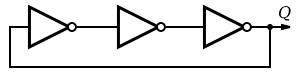
\includegraphics[width=\linewidth]{images/ringoscilatortheorie.png}
        \caption{Een ringoscillator van drie inverters \cite{wikipedia}}
        \label{fig:ringoscillator drie inverters}
\end{figure}
Als de ingang van de eerste inverter hoog is, zal er aan de uitgang van het circuit een laag signaal worden waargenomen. Dit uitgangssignaal wordt dan weer teruggevoerd naar de ingang van het circuit. Hierdoor zal het volgende uitgangssignaal hoog worden en zo verder. Een ringoscillator zou men kunnen gebruiken voor het maken van een kloksignaal, omdat er (zo als net is uitgelegd) een constant signaal van afwisselend hoog en laag wordt waargenomen aan de uitgang. De frequentie van het signaal is afhankelijk van de delay van de oscillator. De delay van de oscillator bestaat uit de opgetelde waarde van de vertragingstijden van de afzonderlijke inverters. Door meer inverters toe te voegen zal de delay groter worden, waardoor de frequentie van de oscillator juist kleiner zal worden. De periode tijd is als volgt:
\begin{equation}
T= 2*t_{p}*N 
\end{equation}\cite[368]{rabaey-integrated-circuits}
\\en
\begin{equation}
t_{p}=(T_{pHL}+T_{pLH})/2 
\end{equation}\cite[28]{rabaey-integrated-circuits}
\\Hierin staat N voor het aantal inverters, $T_{pHL}$ is de high-to-low propegatietijd en $T_{pLH}$ is dan de low-to-high propegatietijd. 


\section{Simulaties}
Voor de simulaties hebben wij een schema gemaakt in PSPICE. Een ringoscillator is een oscillator die enkel uit inverters bestaat. Een inverter is eenvoudig op te bouwen uit twee MOS transistoren. Een inverter is in feite niets anders dan een PMOS transistor bovenop een NMOS transistor. Wij hebben dezelfde MOS transistoren gebruikt als in opdracht 4. De technische specificaties die wij hiervoor hebben gebruikt zijn:
\begin{itemize}
        \item Nominale $V_{DD}$ : 5 V
        \item Minimale kanaallengte: 1.6  \micro\meter\
        \item Maximale kanaallengte: 4.8 \micro\meter\
        \item Minimale kanaalbreedte: 2.4 \micro\meter\
        \item Maximale kanaalbreedte: 10000 \micro\meter\
\end{itemize}
Omdat we gebruik maken van de Sea-of-Gates Chip hebben wij ervoor gekozen om een NMOS transistor van 1.6 x 23.2 \micro\meter\ en PMOS transistor van 1.6 x 29.6 \micro\meter\ te gebruiken.

Een ringoscillator is een schakeling van inverters. Al deze inverters worden in serie aangesloten zodat de ingang van de ene inverter de uitgang is van de vorige inverter. En dat zo in een ketting. Je kan zoveel inverters gebruiken als je wilt. De enige voorwaarde: je hebt een oneven aantal inverters nodig. Dit omdat je anders geen oscillatie krijgt. De oscillatie ontstaat doordat het signaal van hoog naar laag (en omgekeerd) veranderd. Wat hierbij ook belangrijk is dat je geen ideale inverters gebruikt. Bij ideale inverters zou je waarschijnlijk wel een soort van oscillatie krijgen, waarvan de frequentie dan oneindig hoog is. Omdat inverters in werkelijkheid een delay tijd hebben kan je mooiere oscillaties vormen. Hieronder een afbeelding van onze schakeling.
\begin{figure}[H]
\centering
        \includegraphics[width=\linewidth]{images/ringoscillator2.png}
        \caption{De schematische schakeling van de ringoscillator in SPICE}
        \label{fig:schema}
\end{figure}
Vervolgens hebben wij dit schema voor 5\nano\second\  laten lopen. We hebben het Voltage gemeten op het punt waar in figuur \ref{fig:schema} {\it meet} staat. De verkregen data hiervan wordt vermeld in het volgende hoofdstuk. We hebben dit gedaan voor een schakeling van drie inverters en vijf inverters. Zeven inverters was ook een optie om te meten, maar helaas kon PSPICE dit niet simuleren, omdat het circuit 'te groot' zou zijn. In onze conclusie is te lezen dat zeven inverters waarschijnlijk geen (betere/) betrouwbaardere ringoscillator zou vormen.

\section{Resultaten}
Het resultaat van de simulatie van ons circuit met drie inverters ziet er als volgt uit.
\begin{figure}[H]
\centering
                \setlength\figureheight{0.6\textwidth} 
                \setlength\figurewidth{0.9\textwidth}
                % This file was created by matlab2tikz v0.4.2.
% Copyright (c) 2008--2013, Nico Schlömer <nico.schloemer@gmail.com>
% All rights reserved.
% 
% The latest updates can be retrieved from
%   http://www.mathworks.com/matlabcentral/fileexchange/22022-matlab2tikz
% where you can also make suggestions and rate matlab2tikz.
% 
% 
% 
\begin{tikzpicture}

\begin{axis}[%
width=\figurewidth,
height=\figureheight,
scale only axis,
xmin=0,
xmax=5e-09,
xlabel={t (s)},
ymin=-1,
ymax=5,
ylabel={$\text{V}_{\text{meet}}\text{ (V)}$}
]
\addplot [
color=blue,
solid,
line width=2.0pt,
forget plot
]
table[row sep=crcr]{
0 4.99998807907104\\
1e-12 4.93388271331787\\
2e-12 4.86797046661377\\
4.00016074813902e-12 4.73756456375122\\
8.00048224441707e-12 4.47869825363159\\
1.60011252369732e-11 3.99337029457092\\
3.20024112220854e-11 3.23175525665283\\
4.08674379792064e-11 2.8566210269928\\
5.85974914934486e-11 2.1806480884552\\
9.4057598521933e-11 1.14972019195557\\
1.30286046674475e-10 0.561927974224091\\
1.67550591191277e-10 0.240759879350662\\
1.92870923688635e-10 0.157777100801468\\
2.23371738007292e-10 0.106878936290741\\
2.78185892289504e-10 0.0180031787604094\\
3.12132600134239e-10 -0.0368141271173954\\
3.4494425859116e-10 -0.0344616137444973\\
3.78500975107774e-10 0.0700224712491035\\
4.25142773797736e-10 0.600038290023804\\
4.62640148958191e-10 1.30284547805786\\
4.8627828005515e-10 1.75014662742615\\
5.12049721924588e-10 2.19045782089233\\
5.54622805116698e-10 2.80948114395142\\
5.87166708333418e-10 3.23647713661194\\
6.23854997007176e-10 3.6465847492218\\
6.66951949147508e-10 3.97740459442139\\
7.1748784035258e-10 4.35726833343506\\
7.66114520279691e-10 4.58604574203491\\
7.97890082372353e-10 4.54972648620605\\
8.32971839604899e-10 4.30074882507324\\
8.71482028065249e-10 3.65895414352417\\
9.12902599571273e-10 2.65171933174133\\
9.58875010160729e-10 1.57315707206726\\
1.00293238870613e-09 0.821693003177643\\
1.05405035652034e-09 0.310510128736496\\
1.08967926576547e-09 0.16212585568428\\
1.13178668767028e-09 0.061276625841856\\
1.16413268483989e-09 0.00579596823081374\\
1.19716553240828e-09 -0.00853530317544937\\
1.23164192996733e-09 0.0732164233922958\\
1.28265512399189e-09 0.594511151313782\\
1.31881372295134e-09 1.24161505699158\\
1.35309803522937e-09 1.86613619327545\\
1.38992020152323e-09 2.45276618003845\\
1.43145718835108e-09 3.01790189743042\\
1.46457152664475e-09 3.4407594203949\\
1.49569516293518e-09 3.74640560150146\\
1.53010171130113e-09 3.99381303787231\\
1.56776206791215e-09 4.2769775390625\\
1.59977628141455e-09 4.49366426467896\\
1.63024217113666e-09 4.58542585372925\\
1.66092924997024e-09 4.52487659454346\\
1.70254772752337e-09 4.14794063568115\\
1.73546415976994e-09 3.51908898353577\\
1.76778687387519e-09 2.7308042049408\\
1.80276967808418e-09 1.88881456851959\\
1.85332885235362e-09 0.940304696559906\\
1.88928954526596e-09 0.495060652494431\\
1.92346326298825e-09 0.254840850830078\\
1.95984305105917e-09 0.133218184113503\\
2.0015313778054e-09 0.0354394726455212\\
2.0339530449342e-09 -0.0125895282253623\\
2.06437818929367e-09 -0.00135960115585476\\
2.09730626307242e-09 0.111469455063343\\
2.13847654163651e-09 0.568601727485657\\
2.17055478356592e-09 1.15712928771973\\
2.2028600353729e-09 1.76809251308441\\
2.23416993617825e-09 2.29108572006226\\
2.2764461602997e-09 2.8865122795105\\
2.30598654821329e-09 3.27644538879395\\
2.33625453188829e-09 3.61326670646667\\
2.36684265769832e-09 3.8645920753479\\
2.41202344409935e-09 4.18551254272461\\
2.44005625359528e-09 4.40369939804077\\
2.46811234615557e-09 4.56076192855835\\
2.4987004719656e-09 4.59092950820923\\
2.53581949733012e-09 4.40960168838501\\
2.57762423939817e-09 3.81803250312805\\
2.6232765078526e-09 2.74687671661377\\
2.66459230556898e-09 1.76631462574005\\
2.71878363787942e-09 0.822509050369263\\
2.76868506558053e-09 0.32285013794899\\
2.8077249437552e-09 0.156499430537224\\
2.8505017537605e-09 0.0526504851877689\\
2.88053108602576e-09 0.000353319919668138\\
2.91035669147782e-09 -0.0121677555143833\\
2.94072362817638e-09 0.0489650070667267\\
2.98631186820381e-09 0.39527902007103\\
3.01504899039678e-09 0.892581522464752\\
3.03368999380432e-09 1.25650429725647\\
3.05591949950718e-09 1.68655967712402\\
3.09419685732387e-09 2.3297221660614\\
3.13222974296473e-09 2.86401462554932\\
3.16576317641698e-09 3.31014060974121\\
3.19625234920345e-09 3.64330363273621\\
3.22881953548454e-09 3.90122151374817\\
3.27738800775074e-09 4.25552845001221\\
3.30897730532848e-09 4.47884464263916\\
3.32804613504373e-09 4.56698942184448\\
3.35088973156922e-09 4.59999179840088\\
3.38566298819892e-09 4.47408676147461\\
3.43285775966756e-09 3.87234091758728\\
3.46995932273381e-09 3.02680158615112\\
3.505145853756e-09 2.16588616371155\\
3.54814967363887e-09 1.23607909679413\\
3.57934897988849e-09 0.743699729442596\\
3.60937831215374e-09 0.41213858127594\\
3.64334248229675e-09 0.214798718690872\\
3.68416933566146e-09 0.0983957573771477\\
3.72447814084403e-09 0.0112007213756442\\
3.77733069695346e-09 -0.00445675291121006\\
3.83081771656685e-09 0.267675399780273\\
3.87020684070699e-09 0.882762134075165\\
3.9079370465111e-09 1.58690023422241\\
3.94014334529452e-09 2.13772034645081\\
3.98292015529983e-09 2.76423120498657\\
4.01837444156222e-09 3.24284648895264\\
4.05717566832714e-09 3.66941404342651\\
4.10722261518054e-09 4.03795099258423\\
4.1485500544291e-09 4.35533285140991\\
4.19744448959641e-09 4.56131362915039\\
4.23083240389638e-09 4.51696348190308\\
4.27417964897864e-09 4.15501356124878\\
4.30663041993789e-09 3.5615565776825\\
4.3421429138612e-09 2.70736908912659\\
4.3804843001049e-09 1.79480421543121\\
4.43497831225209e-09 0.834488153457642\\
4.4835351429861e-09 0.30808562040329\\
4.51617217846029e-09 0.165566056966782\\
4.55196988992207e-09 0.0805851072072983\\
4.58836714029126e-09 0.0127989426255226\\
4.62808222733252e-09 -0.00754529424011707\\
4.69294884465449e-09 0.296219408512115\\
4.7361272875201e-09 0.983154892921448\\
4.7765525080245e-09 1.72343277931213\\
4.81059234812669e-09 2.28364157676697\\
4.85390466861241e-09 2.88966012001038\\
4.88331117890589e-09 3.28792881965637\\
4.90210643261485e-09 3.50647974014282\\
4.9244378017243e-09 3.72049999237061\\
4.96074774060212e-09 3.98512673377991\\
5.00000000001e-09 4.28657531738281\\
};
\end{axis}
\end{tikzpicture}%
                \caption{Het resultaat van de simulatie met drie inverters.}
                \label{fig:meetdrie}
\end{figure}
En het resultaat van de simulatie met vijf inverters is zoals in figuur \ref{fig:meetvijf}.
\begin{figure}[H]
\centering
                \setlength\figureheight{0.6\textwidth} 
                \setlength\figurewidth{0.9\textwidth}
                % This file was created by matlab2tikz v0.4.2.
% Copyright (c) 2008--2013, Nico Schlömer <nico.schloemer@gmail.com>
% All rights reserved.
% 
% The latest updates can be retrieved from
%   http://www.mathworks.com/matlabcentral/fileexchange/22022-matlab2tikz
% where you can also make suggestions and rate matlab2tikz.
% 
% 
% 
\begin{tikzpicture}

\begin{axis}[%
width=\figurewidth,
height=\figureheight,
scale only axis,
xmin=0,
xmax=5e-09,
xlabel={t (s)},
ymin=-1,
ymax=6,
ylabel={$\text{V}_{\text{meet}}\text{ (V)}$}
]
\addplot [
color=blue,
solid,
line width=2.0pt,
forget plot
]
table[row sep=crcr]{
0 4.99998807907104\\
1e-12 4.9354453086853\\
2e-12 4.87093925476074\\
4.00016074813902e-12 4.74276828765869\\
8.00048224441707e-12 4.48605442047119\\
1.60011252369732e-11 4.00183916091919\\
3.20024112220854e-11 3.23101568222046\\
4.23560989070684e-11 2.78829789161682\\
6.16548488829285e-11 2.05126404762268\\
1.00252348834649e-10 0.998073220252991\\
1.31370164358988e-10 0.510732471942902\\
1.63413481691852e-10 0.241725221276283\\
1.88122633749619e-10 0.169235035777092\\
2.18472108149901e-10 0.142159193754196\\
2.70992880592123e-10 0.119756050407887\\
3.12262112179771e-10 0.108094565570354\\
3.57861993739381e-10 0.0919580385088921\\
3.95336085835472e-10 0.0709834173321724\\
4.42600706497207e-10 0.0676022991538048\\
4.91722151542082e-10 0.0529672689735889\\
5.2469097068347e-10 0.0277629531919956\\
5.64528293812647e-10 -0.0191090945154428\\
6.14313306191936e-10 -0.114129543304443\\
6.59272903481498e-10 -0.150958314538002\\
7.01362863088027e-10 -0.0292072053998709\\
7.43586700314656e-10 0.371628761291504\\
7.72428596297279e-10 0.886534452438354\\
7.99198299551383e-10 1.39601600170136\\
8.26942981125787e-10 1.89386630058289\\
8.65412424223497e-10 2.49429965019226\\
9.18200951905921e-10 3.14536046981812\\
9.54208210946992e-10 3.55337738990784\\
9.88335362540558e-10 3.82852816581726\\
1.02299802461453e-09 4.00887060165405\\
1.05965138869174e-09 4.19881391525269\\
1.09137456388958e-09 4.35612678527832\\
1.11874671643414e-09 4.48414754867554\\
1.14769047582336e-09 4.60842037200928\\
1.19089220175333e-09 4.74335193634033\\
1.23526972243376e-09 4.82735776901245\\
1.27476944112964e-09 4.88118457794189\\
1.31114922920056e-09 4.93400955200195\\
1.35137654365785e-09 5.01091718673706\\
1.38333837026544e-09 5.11539268493652\\
1.41776238092966e-09 5.17829465866089\\
1.44377247420885e-09 5.14630460739136\\
1.4774397852812e-09 4.97674322128296\\
1.52545528476872e-09 4.43632173538208\\
1.56489679580368e-09 3.56890511512756\\
1.60568872457184e-09 2.50798296928406\\
1.64890791280009e-09 1.47286462783813\\
1.69429824678041e-09 0.733065962791443\\
1.74297731360234e-09 0.292019546031952\\
1.7757656889949e-09 0.191748782992363\\
1.81595225808956e-09 0.146901860833168\\
1.864218050519e-09 0.119285091757774\\
1.90874691111781e-09 0.105547919869423\\
1.95031882254221e-09 0.0805407539010048\\
1.99193147932924e-09 0.0691400617361069\\
2.01976638277806e-09 0.0711128935217857\\
2.03612564587779e-09 0.0677066296339035\\
2.05655362447538e-09 0.0572441890835762\\
2.08792173294164e-09 0.0288857463747263\\
2.13317236853577e-09 -0.0280151106417179\\
2.18332990994491e-09 -0.127039596438408\\
2.24265515794791e-09 -0.111576341092587\\
2.28667179113068e-09 0.126456871628761\\
2.32435543080606e-09 0.679291069507599\\
2.36479229284264e-09 1.42407429218292\\
2.39500788962282e-09 1.95634615421295\\
2.43384404098429e-09 2.55054807662964\\
2.48209819188155e-09 3.14298295974731\\
2.51437433985807e-09 3.5153534412384\\
2.54457829510607e-09 3.77712464332581\\
2.5747589672897e-09 3.95032048225403\\
2.62571977441944e-09 4.21519565582275\\
2.66112167378701e-09 4.38641262054443\\
2.69569120360352e-09 4.54005527496338\\
2.72928284471668e-09 4.66883659362793\\
2.77624478554167e-09 4.78941917419434\\
2.81582017419674e-09 4.84922552108765\\
2.85834669126011e-09 4.906822681427\\
2.89958099825121e-09 4.97464847564697\\
2.94533804049529e-09 5.10416173934937\\
2.99617661153711e-09 5.14996337890625\\
3.02981481877901e-09 5.03955459594727\\
3.06992571791448e-09 4.710045337677\\
3.11779569824971e-09 3.87903571128845\\
3.1638787033949e-09 2.69917464256287\\
3.20567762469687e-09 1.67705678939819\\
3.25762796206214e-09 0.7861328125\\
3.29953747791983e-09 0.361568421125412\\
3.33968912241794e-09 0.198937460780144\\
3.37665098709799e-09 0.151064455509186\\
3.4291834010724e-09 0.118042550981045\\
3.47066800100543e-09 0.106937535107136\\
3.51005712514557e-09 0.0839054584503174\\
3.55575595972873e-09 0.0687326565384865\\
3.58643721779622e-09 0.0707624182105064\\
3.60518881575949e-09 0.0664270520210266\\
3.62783741662092e-09 0.0539550185203552\\
3.65849539162405e-09 0.0251042526215315\\
3.70414183931239e-09 -0.0368057303130627\\
3.75412475773878e-09 -0.135444119572639\\
3.80582480216213e-09 -0.122971333563328\\
3.84627912649698e-09 0.0685292556881905\\
3.88567407140322e-09 0.602746486663818\\
3.931157537641e-09 1.43206191062927\\
3.96336383642442e-09 1.99516463279724\\
4.00154806198366e-09 2.57412266731262\\
4.05054727094062e-09 3.17413926124573\\
4.08491307394393e-09 3.56111145019531\\
4.11846396969445e-09 3.82990646362305\\
4.15285887652822e-09 4.01401042938232\\
4.1899371565301e-09 4.19771432876587\\
4.22434952566214e-09 4.36926031112671\\
4.25541495429166e-09 4.51514101028442\\
4.28504265369661e-09 4.63598966598511\\
4.33344814451225e-09 4.77505970001221\\
4.38310510003753e-09 4.85609769821167\\
4.43186565758474e-09 4.91850614547729\\
4.4728613131661e-09 4.99057102203369\\
4.50986392320879e-09 5.10342264175415\\
4.55417741546221e-09 5.16555166244507\\
4.58633132735081e-09 5.0874457359314\\
4.62352602267452e-09 4.83009386062622\\
4.67305492134579e-09 4.09351491928101\\
4.70587822133489e-09 3.2943639755249\\
4.73720558443852e-09 2.47249865531921\\
4.76854458907433e-09 1.68816745281219\\
4.81376030007191e-09 0.862598419189453\\
4.84657777929492e-09 0.473195225000381\\
4.87624622406252e-09 0.278573364019394\\
4.90664226459153e-09 0.210722774267197\\
4.9511944082547e-09 0.156326666474342\\
4.99661384606548e-09 0.124193333089352\\
5.00000000001e-09 0.123630166053772\\
};
\end{axis}
\end{tikzpicture}%
                \caption{Het resultaat van de simulatie met vijf inverters.}
                \label{fig:meetvijf}
\end{figure}
Aan alleen deze plots hadden we niet zoveel om de vraag {\it 'Wat is het kleinst aantal inverters waarbij een betrouwbare oscillatie optreed?'} te beantwoorden. Om deze vraag wel te kunnen beantwoorden hebben we nog een extra plot gemaakt, zie figuur \ref{fig:tplhtphl5}. Uit deze plot hebben we de $T_{pHL}$ en $T_{pLH}$ waarde van onze simulatie afgelezen. De $T_{pHL}$ waarde vonden we door bij de eerste opgaande flank van de blauwe golf op ongeveer 50\% van de golf een horizontale lijn (helaas konden we die niet weergeven in de figuur) te tekenen tot er een raakpunt is met de rode lijn. Door vervolgens de resultaten van elkaar af te halen vonden we een $T_{pHL}$ van 0.107\nano\second\ . Om nu vervolgens de waarde van $T_{pLH}$ te vinden hebben we wederom een horizontale lijn getrokken met het beginpunt op 50\% van de neergaande flank van de eerste blauwe golf en het eindpunt op de opgaande flank van de tweede rode golf. Dit gaf ons een waarde van 0.21\nano\second\ voor $T_{pLH}$.

\begin{figure}[H]
\centering
                \setlength\figureheight{0.6\textwidth} 
                \setlength\figurewidth{0.9\textwidth}
                % This file was created by matlab2tikz v0.4.2.
% Copyright (c) 2008--2013, Nico Schlömer <nico.schloemer@gmail.com>
% All rights reserved.
% 
% The latest updates can be retrieved from
%   http://www.mathworks.com/matlabcentral/fileexchange/22022-matlab2tikz
% where you can also make suggestions and rate matlab2tikz.
% 
% 
% 
\begin{tikzpicture}

\begin{axis}[%
width=\figurewidth,
height=\figureheight,
scale only axis,
xmin=0,
xmax=5e-09,
xlabel={t(s)},
ymin=-1,
ymax=6,
ylabel={$\text{V}_{\text{meet}}\text{ (V)}$},
legend style={at={(0.721078431372549,0.799328295549958)},anchor=south west,draw=black,fill=white,legend cell align=left}
]
\addplot [
color=blue,
solid,
line width=2.0pt
]
table[row sep=crcr]{
0 1.33496280696477e-09\\
1e-12 -0.0170593522489071\\
2e-12 -0.0335659310221672\\
4.00016074813902e-12 -0.0644001066684723\\
8.00048224441707e-12 -0.122534789144993\\
1.60011252369732e-11 -0.214187189936638\\
3.20024112220854e-11 -0.301287800073624\\
4.23560989070684e-11 -0.317778050899506\\
6.16548488829285e-11 -0.288125932216644\\
1.00252348834649e-10 -0.0152324307709932\\
1.31370164358988e-10 0.536688029766083\\
1.63413481691852e-10 1.19139862060547\\
1.88122633749619e-10 1.679891705513\\
2.18472108149901e-10 2.21148228645325\\
2.70992880592123e-10 2.93905329704285\\
3.12262112179771e-10 3.41782569885254\\
3.57861993739381e-10 3.82327270507813\\
3.95336085835472e-10 4.02465152740479\\
4.42600706497207e-10 4.26587295532227\\
4.91722151542082e-10 4.48933124542236\\
5.2469097068347e-10 4.62344455718994\\
5.64528293812647e-10 4.74626445770264\\
6.14313306191936e-10 4.83909225463867\\
6.59272903481498e-10 4.89913415908813\\
7.01362863088027e-10 4.96246290206909\\
7.43586700314656e-10 5.06018018722534\\
7.72428596297279e-10 5.14908838272095\\
7.99198299551383e-10 5.17775011062622\\
8.26942981125787e-10 5.12014389038086\\
8.65412424223497e-10 4.87442207336426\\
9.18200951905921e-10 4.1103401184082\\
9.54208210946992e-10 3.22911262512207\\
9.88335362540558e-10 2.34381437301636\\
1.02299802461453e-09 1.49375081062317\\
1.05965138869174e-09 0.848480522632599\\
1.09137456388958e-09 0.472318679094315\\
1.11874671643414e-09 0.288664817810059\\
1.14769047582336e-09 0.218022778630257\\
1.19089220175333e-09 0.161973506212235\\
1.23526972243376e-09 0.12746986746788\\
1.27476944112964e-09 0.112583070993423\\
1.31114922920056e-09 0.0893329009413719\\
1.35137654365785e-09 0.0701308026909828\\
1.38333837026544e-09 0.0723109543323517\\
1.41776238092966e-09 0.0649147555232048\\
1.44377247420885e-09 0.0482479818165302\\
1.4774397852812e-09 0.0134492935612798\\
1.52545528476872e-09 -0.0561151616275311\\
1.56489679580368e-09 -0.139891251921654\\
1.60568872457184e-09 -0.143477618694305\\
1.64890791280009e-09 0.0314050577580929\\
1.69429824678041e-09 0.625820517539978\\
1.74297731360234e-09 1.50623345375061\\
1.7757656889949e-09 2.06817555427551\\
1.81595225808956e-09 2.65955591201782\\
1.864218050519e-09 3.242915391922\\
1.90874691111781e-09 3.70163226127625\\
1.95031882254221e-09 3.96291375160217\\
1.99193147932924e-09 4.17782068252563\\
2.01976638277806e-09 4.30993986129761\\
2.03612564587779e-09 4.38753747940063\\
2.05655362447538e-09 4.48336124420166\\
2.08792173294164e-09 4.61451530456543\\
2.13317236853577e-09 4.75284814834595\\
2.18332990994491e-09 4.84280729293823\\
2.24265515794791e-09 4.9267520904541\\
2.28667179113068e-09 5.00479507446289\\
2.32435543080606e-09 5.11875200271606\\
2.36479229284264e-09 5.16677951812744\\
2.39500788962282e-09 5.09270429611206\\
2.43384404098429e-09 4.82371950149536\\
2.48209819188155e-09 4.10756587982178\\
2.51437433985807e-09 3.32479000091553\\
2.54457829510607e-09 2.53165102005005\\
2.5747589672897e-09 1.77315235137939\\
2.62571977441944e-09 0.844512283802032\\
2.66112167378701e-09 0.442403525114059\\
2.69569120360352e-09 0.245911106467247\\
2.72928284471668e-09 0.19316703081131\\
2.77624478554167e-09 0.145548090338707\\
2.81582017419674e-09 0.12332509458065\\
2.85834669126011e-09 0.102001160383224\\
2.89958099825121e-09 0.0757316052913666\\
2.94533804049529e-09 0.0705234855413437\\
2.99617661153711e-09 0.0538459084928036\\
3.02981481877901e-09 0.0272757578641176\\
3.06992571791448e-09 -0.021054619923234\\
3.11779569824971e-09 -0.114024102687836\\
3.1638787033949e-09 -0.161999434232712\\
3.20567762469687e-09 -0.0320391096174717\\
3.25762796206214e-09 0.5719895362854\\
3.29953747791983e-09 1.32608687877655\\
3.33968912241794e-09 2.02478241920471\\
3.37665098709799e-09 2.57876324653625\\
3.4291834010724e-09 3.22030138969421\\
3.47066800100543e-09 3.66052341461182\\
3.51005712514557e-09 3.92531538009644\\
3.55575595972873e-09 4.16316413879395\\
3.58643721779622e-09 4.30900049209595\\
3.60518881575949e-09 4.3977632522583\\
3.62783741662092e-09 4.50333118438721\\
3.65849539162405e-09 4.62855052947998\\
3.70414183931239e-09 4.7619514465332\\
3.75412475773878e-09 4.84663105010986\\
3.80582480216213e-09 4.91899633407593\\
3.84627912649698e-09 4.98850440979004\\
3.88567407140322e-09 5.10531759262085\\
3.931157537641e-09 5.16194343566895\\
3.96336383642442e-09 5.07703447341919\\
4.00154806198366e-09 4.80167055130005\\
4.05054727094062e-09 4.04222726821899\\
4.08491307394393e-09 3.19904112815857\\
4.11846396969445e-09 2.33038902282715\\
4.15285887652822e-09 1.5052285194397\\
4.1899371565301e-09 0.814030528068542\\
4.22434952566214e-09 0.418652445077896\\
4.25541495429166e-09 0.245628744363785\\
4.28504265369661e-09 0.185038521885872\\
4.33344814451225e-09 0.140055373311043\\
4.38310510003753e-09 0.116169601678848\\
4.43186565758474e-09 0.0963209122419357\\
4.4728613131661e-09 0.0737712681293488\\
4.50986392320879e-09 0.0725162848830223\\
4.55417741546221e-09 0.059477299451828\\
4.58633132735081e-09 0.0356579497456551\\
4.62352602267452e-09 -0.00666845683008432\\
4.67305492134579e-09 -0.0931844189763069\\
4.70587822133489e-09 -0.152272716164589\\
4.73720558443852e-09 -0.142783537507057\\
4.76854458907433e-09 -0.0378559306263924\\
4.81376030007191e-09 0.436054170131683\\
4.84657777929492e-09 1.02915191650391\\
4.87624622406252e-09 1.58959424495697\\
4.90664226459153e-09 2.12098550796509\\
4.9511944082547e-09 2.76068997383118\\
4.99661384606548e-09 3.2972948551178\\
5.00000000001e-09 3.33752059936523\\
};
\addlegendentry{meetpunt1};

\addplot [
color=red,
solid,
line width=2.0pt
]
table[row sep=crcr]{
0 5\\
1e-12 4.99440145492554\\
2e-12 4.9890718460083\\
4.00016074813902e-12 4.97943878173828\\
8.00048224441707e-12 4.96187925338745\\
1.60011252369732e-11 4.93753147125244\\
3.20024112220854e-11 4.92391157150269\\
4.23560989070684e-11 4.92853307723999\\
6.16548488829285e-11 4.95254945755005\\
1.00252348834649e-10 5.03452730178833\\
1.31370164358988e-10 5.15449094772339\\
1.63413481691852e-10 5.22681522369385\\
1.88122633749619e-10 5.2070426940918\\
2.18472108149901e-10 5.07203245162964\\
2.70992880592123e-10 4.51886749267578\\
3.12262112179771e-10 3.62047839164734\\
3.57861993739381e-10 2.43238186836243\\
3.95336085835472e-10 1.5250369310379\\
4.42600706497207e-10 0.7386554479599\\
4.91722151542082e-10 0.290259957313538\\
5.2469097068347e-10 0.189842745661736\\
5.64528293812647e-10 0.146438702940941\\
6.14313306191936e-10 0.118443384766579\\
6.59272903481498e-10 0.104666352272034\\
7.01362863088027e-10 0.0795673653483391\\
7.43586700314656e-10 0.0691606104373932\\
7.72428596297279e-10 0.0691429153084755\\
7.99198299551383e-10 0.0597331374883652\\
8.26942981125787e-10 0.0391823314130306\\
8.65412424223497e-10 -0.00331376725807786\\
9.18200951905921e-10 -0.0924475342035294\\
9.54208210946992e-10 -0.153894811868668\\
9.88335362540558e-10 -0.130402505397797\\
1.02299802461453e-09 0.0113984933122993\\
1.05965138869174e-09 0.433043152093887\\
1.09137456388958e-09 1.01069414615631\\
1.11874671643414e-09 1.53342318534851\\
1.14769047582336e-09 2.04784512519836\\
1.19089220175333e-09 2.68567442893982\\
1.23526972243376e-09 3.21521210670471\\
1.27476944112964e-09 3.6388943195343\\
1.31114922920056e-09 3.89446640014648\\
1.35137654365785e-09 4.1002025604248\\
1.38333837026544e-09 4.25717687606812\\
1.41776238092966e-09 4.4220871925354\\
1.44377247420885e-09 4.54151678085327\\
1.4774397852812e-09 4.67038202285767\\
1.52545528476872e-09 4.7941722869873\\
1.56489679580368e-09 4.85330963134766\\
1.60568872457184e-09 4.90815782546997\\
1.64890791280009e-09 4.97951316833496\\
1.69429824678041e-09 5.10947847366333\\
1.74297731360234e-09 5.15294361114502\\
1.7757656889949e-09 5.04859495162964\\
1.81595225808956e-09 4.72532558441162\\
1.864218050519e-09 3.8991105556488\\
1.90874691111781e-09 2.77213311195374\\
1.95031882254221e-09 1.75153303146362\\
1.99193147932924e-09 0.966824948787689\\
2.01976638277806e-09 0.567352175712585\\
2.03612564587779e-09 0.409453988075256\\
2.05655362447538e-09 0.289109587669373\\
2.08792173294164e-09 0.203316077589989\\
2.13317236853577e-09 0.149312153458595\\
2.18332990994491e-09 0.118843838572502\\
2.24265515794791e-09 0.0931184515357018\\
2.28667179113068e-09 0.0703339949250221\\
2.32435543080606e-09 0.0697208791971207\\
2.36479229284264e-09 0.0571272373199463\\
2.39500788962282e-09 0.0349454656243324\\
2.43384404098429e-09 -0.00856954697519541\\
2.48209819188155e-09 -0.0921069532632828\\
2.51437433985807e-09 -0.151781871914864\\
2.54457829510607e-09 -0.147389084100723\\
2.5747589672897e-09 -0.0557106100022793\\
2.62571977441944e-09 0.474450916051865\\
2.66112167378701e-09 1.1112539768219\\
2.69569120360352e-09 1.74773728847504\\
2.72928284471668e-09 2.30938267707825\\
2.77624478554167e-09 2.93565678596497\\
2.81582017419674e-09 3.39728355407715\\
2.85834669126011e-09 3.78541684150696\\
2.89958099825121e-09 4.01583957672119\\
2.94533804049529e-09 4.25249195098877\\
2.99617661153711e-09 4.48660326004028\\
3.02981481877901e-09 4.62393379211426\\
3.06992571791448e-09 4.74720478057861\\
3.11779569824971e-09 4.83657550811768\\
3.1638787033949e-09 4.89474248886108\\
3.20567762469687e-09 4.9600887298584\\
3.25762796206214e-09 5.09830951690674\\
3.29953747791983e-09 5.16162776947021\\
3.33968912241794e-09 5.06204175949097\\
3.37665098709799e-09 4.78780651092529\\
3.4291834010724e-09 3.93725776672363\\
3.47066800100543e-09 2.89280700683594\\
3.51005712514557e-09 1.9116849899292\\
3.55575595972873e-09 1.01548290252686\\
3.58643721779622e-09 0.565773665904999\\
3.60518881575949e-09 0.389225393533707\\
3.62783741662092e-09 0.268460929393768\\
3.65849539162405e-09 0.19571940600872\\
3.70414183931239e-09 0.155865415930748\\
3.75412475773878e-09 0.12402531504631\\
3.80582480216213e-09 0.0975072085857391\\
3.84627912649698e-09 0.0729753896594048\\
3.88567407140322e-09 0.0705975517630577\\
3.931157537641e-09 0.0572236701846123\\
3.96336383642442e-09 0.0333758816123009\\
4.00154806198366e-09 -0.0103069823235273\\
4.05054727094062e-09 -0.0988126397132874\\
4.08491307394393e-09 -0.15446849167347\\
4.11846396969445e-09 -0.129223302006722\\
4.15285887652822e-09 0.016698956489563\\
4.1899371565301e-09 0.438493251800537\\
4.22434952566214e-09 1.07109308242798\\
4.25541495429166e-09 1.65877115726471\\
4.28504265369661e-09 2.16308665275574\\
4.33344814451225e-09 2.84109735488892\\
4.38310510003753e-09 3.41869783401489\\
4.43186565758474e-09 3.84195470809937\\
4.4728613131661e-09 4.05782413482666\\
4.50986392320879e-09 4.25062322616577\\
4.55417741546221e-09 4.45800971984863\\
4.58633132735081e-09 4.59471940994263\\
4.62352602267452e-09 4.71886014938354\\
4.67305492134579e-09 4.82347393035889\\
4.70587822133489e-09 4.86807489395142\\
4.73720558443852e-09 4.90972423553467\\
4.76854458907433e-09 4.95887184143066\\
4.81376030007191e-09 5.07364463806152\\
4.84657777929492e-09 5.16087913513184\\
4.87624622406252e-09 5.1627345085144\\
4.90664226459153e-09 5.05843925476074\\
4.9511944082547e-09 4.66542863845825\\
4.99661384606548e-09 3.81940364837646\\
5.00000000001e-09 3.73756313323975\\
};
\addlegendentry{meetpunt2};

\end{axis}
\end{tikzpicture}%
                \caption{Figuur gebruikt om de $T_{pLH}$ en $T_{pHL}$ te berekenen.}
                \label{fig:tplhtphl5}
\end{figure}
Aan de hand van deze waarde kunnen we de oscillatiefrequentie berekenen met de volgende formule: 
\begin{equation}
Frequentie = 1/(N*(T_{pHL}+T_{pLH}))
\end{equation}
Hierin staat N wederom voor het aantal inverters. 
\\Voor ons circuit met drie inverters geeft dit ons: 
\begin{equation}
Frequentie = 1/(3*(0.107\nano\second\ + 0.21\nano\second\ )) = 1051.5 MHz
\end{equation} 
\\en voor vijf inverters:
\begin{equation}
Frequentie = 1/(5*(0.107\nano\second\ + 0.21\nano\second\ )) = 630.9 MHz
\end{equation} 
Als sanity-check moesten we dit vergelijken met de gegeven informatie in Appendix D van de EPO3 handleiding. In deze handleiding waren de gegeven waarden voor  $T_{pLH}$ =  0.19\nano\second\ en voor  $T_{pHL}$ = 0.23\nano\second .  De sanity-check levert ons de volgende berekeningen en resultaten op: 
\begin{equation}
Frequentie = 1/(3*(0.23\nano\second\ + 0.19\nano\second\ )) = 793.7 MHz
\end{equation} 
\\en voor vijf inverters:
\begin{equation}
Frequentie = 1/(5*(0.23\nano\second\ + 0.19\nano\second\ )) = 476.2 MHz
\end{equation} 

\section{Conclusie}
Uit onze verkregen resultaten kunnen we het volgende concluderen:
\begin{itemize}
	\item Hoe meer inverters je gebruikt, hoe groter de delay, hoe kleiner de oscillatiefrequentie.
	\item Hoe meer inverters we gebruiken, hoe kleiner het verschil wordt tussen onze gemeten waarde en de waarde verkregen uit de sanity-check.
\end{itemize}
Hierdoor kunnen wij concluderen dat het minst aantal inverters wat nodig is voor een betrouwbare oscillatie zal liggen bij vijf inverters. 


\section{Discussie}
Altijd zijn er natuurlijk een aantal zaken te verbeteren. Bij deze opdracht hebben we ook een aantal punten waar verbetering in zit. Zo waren we uiteraard beperkt door het programma PSPICE die een grens heeft tot waar deze nog kan simuleren. Helaas probeerden wij een schema te simuleren dat boven deze grens lag. Hierdoor missen we resultaten die misschien wel interessant zouden kunnen zijn. 
De grafieken die we hebben gebruikt voor berekeningen en analyses hebben we geanalyseerd in matlab. De oorspronkelijke grafiek kwam uit de simulatie van PSPICE. Deze hebben we moeten extraheren vanuit PSPICE en via notepad moeten implementeren in Matlab. Hier kan uiteraard het een en ander fout zijn gegaan waardoor de grafieken van matlab en PSPICE niet identiek aan elkaar waren. Dit heeft invloed op de resultaten aangezien je met de waarden van matlab verdere conclusies gaat trekken. 
De transistoren die we hebben geimplenteerd in PSPICE zijn immers ook maar simulaties. De resultaten die we uit deze simulaties hebbben verkregen kunnen uiteraard verschillen met de resultaten die te verkrijgen zijn als je deze schakeling in het echt bouwt. Dit heeft opzich niet veel invloed op deze opdracht, aangezien we de transistoren allen theoretisch hoefden te benaderen. 

\newpage
\section{Bibliografie}
\printbibliography
\end{document}